\documentclass[11pt]{article}

\usepackage{amsmath}
\usepackage{amsfonts}
\usepackage{amssymb}
\usepackage{graphicx}
\usepackage[center]{caption}
\usepackage{mathtools}
\usepackage{lipsum}
\usepackage{stackengine}
\usepackage{fancyhdr}
\usepackage{caption}
\usepackage{tikz}
\usetikzlibrary{shapes.geometric, arrows}
\usepackage{float}
\usepackage[a4paper,left=1in,right=1in,top=1in,bottom=1in,footskip=.25in]{geometry}
\usepackage{etoolbox}
\usepackage[nottoc]{tocbibind}
\usepackage{tabu}
\usepackage{enumitem,kantlipsum}
\usepackage{verbatim}
\usepackage{hyperref}
\begin{document}


\section{Aim}
This test case is for checking the computation time taken by each function in the code to find the possible bottleneck of the written Isogeometric analysis code.
\section{Problem description} \label{2DPWLELPD}
\emph{Section 8 in Documentation}\\
A 2D plate is subjected to mechanical loading as shown in Figure(\ref{TimeitLoading}). The material used is PZT-PIC151 ceramics.
The movement of bottom edge AB is fixed in y-direction and left edge AC in x-direction. A displacement of 100 nm (1e-4 mm) is given on the right edge BD and 200nm (2e-4 mm) on top edge CD.
\textbf{The analysis is done for 50 control points in each direction and 2nd order NURBS basis functions, to get a clear picture of the analysis time for each function.}
\begin{figure}[H]
	\centering
	\begin{minipage}{.5\textwidth}
		\centering
		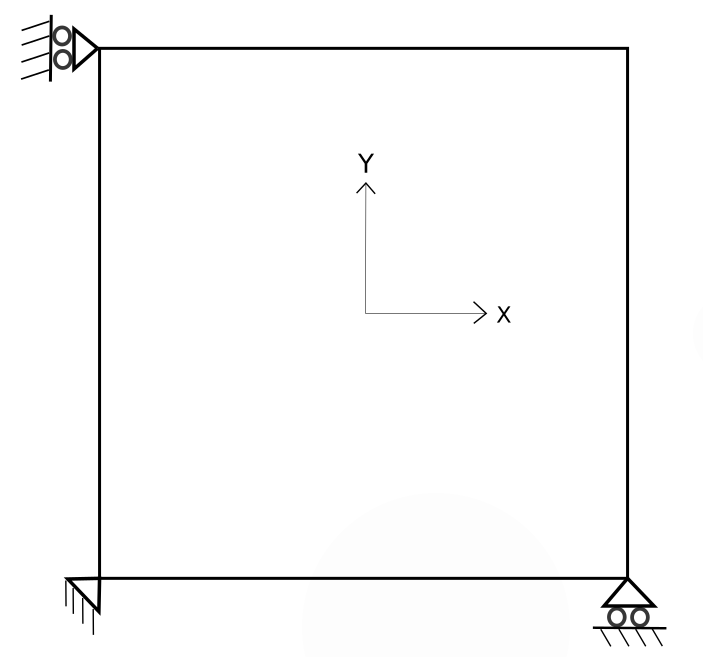
\includegraphics[width=0.8\linewidth]{2DPlate.png}
		\captionof{figure}{2D Plate}
		\label{2Dplate}
	\end{minipage}%
	\begin{minipage}{.5\textwidth}
		\centering
		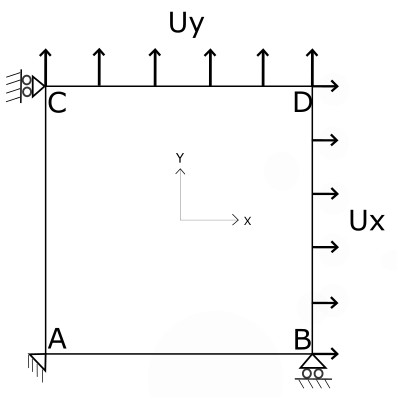
\includegraphics[width=0.9\linewidth]{TimeitLoading.png}
		\captionof{figure}{2D Piezoelectric Plate with loading}
		\label{TimeitLoading}
	\end{minipage}
\end{figure}
\textbf{timeit} package in python is used to compute time taken by a function. A sample code is shown below.
\begin{figure}[H]
	\begin{center}
		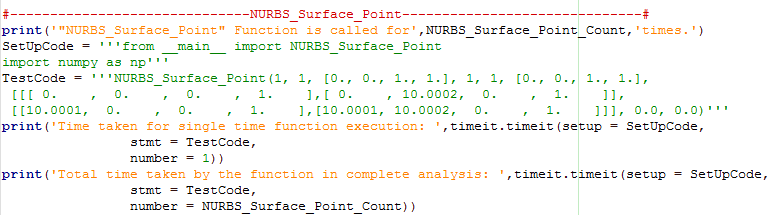
\includegraphics[scale=0.9]{TimeitCode.png} 
		\caption{\\Sample code calculating the computation time of a function}\label{TimeitCode}
	\end{center}	
\end{figure}
\newpage
\section{How to run the Program}
\begin{enumerate}[leftmargin=*]
	\item The code is written in python and external libraries numpy, matplotlib.pyplot, sys, path from pathlib, timeit and math are used.
	\item Please use any environment which will compile python programs
	\item A python file and the generated data file is present in the folder.
	\item Before you run the file, please make sure that the working directory is same as the folder  which
	Consists the Program.
	\item Use command  $>>>$ python Main\_Program.py to run the program.
	\item A "log.txt" file is created which contain the information of the computational times of each function. 
	 
	
\end{enumerate}
\newpage
\section{Findings and Conclusion} \label{Findings}

Below is the data generated by using timeit. The code is written to generate the data regarding number of times each function is called in the program and total time taken by each function in the analysis.\\
From the below values we can see that the time taken by "SurfaceDerivsAlgAuv" Function and "B\_matrix" Function is more when compared to other functions apart from element routine. \\
"SurfaceDerivsAlgAuv" Function is used to compute derivatives of the NURBS bi-variate basis functions.\\ 
Derivatives of basis functions are handled differently in IGA compared to FEM because of the recursive nature of the NURBS basis functions. Optimizing "SurfaceDerivsAlgAuv" function is necessary to reduce overall computation time.\\
\textbf{Program generated data for 50 control points in each direction}

\begin{verbatim}
"KnotVector" Fucntion is called for 2 times.
Time taken for single time function execution:  1.5964999988682393e-05
Total time taken by the function in complete analysis:  3.021800000624353e-05

"FindSpan" Fucntion is called for 120248 times.
Time taken for single time function execution:  1.0263000007171286e-05
Total time taken by the function in complete analysis:  0.44270469899998943

"BasisFuns" Fucntion is called for 158664 times.
Time taken for single time function execution:  3.306900001120994e-05
Total time taken by the function in complete analysis:  2.1537873399999796

"DersBasisFuns" Fucntion is called for 230496 times.
Time taken for single time function execution:  5.302499999970678e-05
Total time taken by the function in complete analysis:  10.28354588900001

"ControlPointAssembly" Fucntion is called for 4802 times.
Time taken for single time function execution:  0.00010034799998948074
Total time taken by the function in complete analysis:  0.25946407300000374

"materialRoutine" Fucntion is called for 19208 times.
Time taken for single time function execution:  7.469100000889739e-05
Total time taken by the function in complete analysis:  0.7070453440000222

"elementRoutine" Fucntion is called for 4802 times.
Time taken for single time function execution:  0.0065517000000170356
Total time taken by the function in complete analysis:  32.14903563299998

"Jacobian12" Fucntion is called for 38424 times.
Time taken for single time function execution:  0.00047551299999781804
Total time taken by the function in complete analysis:  17.596252571999997

"B_matrix" Fucntion is called for 38424 times.
Time taken for single time function execution:  0.0010496630000034202
Total time taken by the function in complete analysis:  37.19408733499998

"NURBS_Surface_Point" Function is called for 2500 times.
Time taken for single time function execution:  6.0437000001911656e-05
Total time taken by the function in complete analysis:  0.11756569399994987

"SurfaceDerivsAlgAuv" Function is called for 153700 time.
Time taken for single time function execution:  0.00040823400001954724
Total time taken by the function in complete analysis:  64.39044447399999

"GaussPoints" Function is called for 1 time.
Time taken for single time function execution:  4.390300000522984e-05
Total time taken by the function in complete analysis:  4.903399997147062e-05
\end{verbatim}



\end{document}